\documentclass{amsart}

\include{RDTP-Preamble}

\begin{document}

\title{The balanced tensor product of module categories}

\begin{abstract}
The balanced tensor product $M \otimes_A N$ of two modules over an algebra $A$ is the vector space corepresenting $A$-balanced bilinear maps out of the product $M \times N$.  The balanced tensor product $\cM \boxtimes_{\cC} \cN$ of two module categories over a monoidal linear category $\cC$ is the linear category corepresenting $\cC$-balanced right-exact bilinear functors out of the product category $\cM \times \cN$.  We show that the balanced tensor product can be realized as a category of bimodule objects in $\cC$, provided the monoidal linear category is finite and rigid.
\end{abstract}




%A key role in the theory of tensor categories is played by the balanced tensor product $\cM \boxtimes_\cC \cN$ which is a higher dimensional analogue of the tensor product of a right and a left module over a non-commutative ring.  The balanced tensor product is characterized by a universal property, but such a characterization does not guarantee existence.  In this paper, we give a construction of the balanced tensor product for finite tensor categories (in the sense of Etingof-Ostrik) and their finite module categories.  This generalizes results of Etingof-Nikshych-Ostrik in the semisimple case.  Explicitly, we realize the balanced tensor product over $\cC$ as a category of bimodule objects in $\cC$.

\author{Christopher L. Douglas}
\address{Mathematical Institute\\ University of Oxford\\ Oxford OX1 3LB\\ United Kingdom}
\email{cdouglas@maths.ox.ac.uk}
\urladdr{http://people.maths.ox.ac.uk/cdouglas}
      	
\author{Christopher Schommer-Pries}
\address{Department of Mathematics\\ Max Planck Institute for Mathematics \\ 53111 Bonn \\ Germany}
\email{schommerpries.chris.math@gmail.com}
\urladdr{http://sites.google.com/site/chrisschommerpriesmath}

\author{Noah Snyder}
\address{Department of Mathematics\\ Indiana University\\ Bloomington, IN 47401\\ USA}
\email{nsnyder@math.indiana.edu}
\urladdr{http://www.math.columbia.edu/\!\raisebox{-1mm}{~}nsnyder/}

\thanks{CD was partially supported by a Miller Research Fellowship and by EPSRC grant EP/K015478/1, CSP was partially supported by NSF fellowship DMS-0902808 and the Max Planck Institute for Mathematics, and NS was partially supported by NSF fellowship DMS-0902981 and DARPA HR0011-11-1-0001.  We thank the referee for suggestions and corrections, and thank Manuel Ara\'ujo for pointing out a simplification of the proof of Theorem~\ref{thm:DelignePrdtOverATCExists}.
}


\maketitle	

\tikzexternaldisable

%\setcounter{tocdepth}{2}
%\tableofcontents

\section{Introduction}

%Intro version 3
Tensor categories are a higher dimensional analogue of algebras.  Just as modules and bimodules play a key role in the theory of algebras, the analogous notions of module categories and bimodule categories play a key role in the study of tensor categories (as pioneered by Ostrik \cite{MR1976459}).  One of the key constructions in the theory of modules and bimodules is the relative tensor product $M \otimes_A N$.  As first recognized by Tambara \cite{tambara}, a similarly important role is played by the balanced tensor product of module categories over a monoidal category $\cM \boxtimes_\cC \cN$ (for example, see \cite{MR1966524, 0909.3140, MR2511638, MR2909758, 1202.4396, MR3022755, MR3063919}).  For $\cC = \Vect$, this agrees with Deligne's~\cite{MR1106898} tensor product $\cK \boxtimes \cL$ of finite linear categories.  Etingof, Nikshych, and Ostrik~\cite{0909.3140} established the existence of a balanced tensor product $\cM \boxtimes_{\cC} \cN$ of finite semisimple module categories over a fusion category, and Davydov and Nikshych \cite[\S 2.7]{MR3107567} outlined how to generalize this construction to module categories over a finite tensor category.\footnote{We were unaware of Davydov--Nikshych's result while writing this paper.}  We give a new construction of the balanced tensor product over a finite tensor category as a category of bimodule objects.

Recall that the balanced tensor product $M \otimes_A N$ of modules is, by definition, the vector space corepresenting $A$-balanced bilinear functions out of $M \times N$.  In other words, giving a map $M \otimes_A N \rightarrow X$ is the same as giving a billinear map $f: M \times N \rightarrow X$ with the property that $f(ma,n) = f(m, an)$.  If the balanced tensor product exists, it is certainly unique (up to unique isomorphism), but the universal property does not guarantee existence.  Instead existence is typically established by an explicit construction as a quotient of a free abelian group on the product $M \times N$. We now describe the balanced tensor product $\cM \boxtimes_{\cC} \cN$ of module categories over a tensor category.  Again this should be universal for certain bilinear functors, however when passing from algebras to tensor categories, the analogue of the equality $f(ma,n) = f(m, an)$ is a natural system of isomorphisms $\eta_{m,a,n}: \cF(m \otimes a,n) \rightarrow \cF(m, a \otimes n)$ satisfying some natural coherence properties.  A bilinear functor $\cF$ together with a natural coherent system of isomorphisms $\eta_{m,a,n}$ is called a $\cC$-balanced functor.  Thus the balanced tensor product $\cM \boxtimes_{\cC} \cN$ is defined to be the linear category corepresenting $\cC$-balanced right-exact bilinear functors out of $\cM \times \cN$. In other words, giving a right-exact functor $\cM \boxtimes_{\cC} \cN \rightarrow \cX$ is the same as giving a right-exact bilinear functor $\cM \times \cN \rightarrow \cX$ together with isomorphisms $\eta_{m,a,n}: \cF(m \otimes a,n) \rightarrow \cF(m, a \otimes n)$ satisfying a coherence property.  Again if the balanced tensor product exists, it is unique (up to an equivalence that is unique up to unique natural isomorphism), but existence does not follow formally. 

The only task is to provide an explicit construction of the balanced tensor product that satisfies the corepresentation property.  A crucial tool for the construction is the result, proved by Etingof--Gelaki--Nikshych--Ostrik \cite[Corollary 7.10.5.]{egno-book}, based on earlier work of Etingof--Ostrik \cite[\S 3.2]{EO-ftc} along the lines pioneered by Ostrik \cite[Thm 1]{MR1976459}, that any finite left module category ${}_{\cC} \cN$ over a finite tensor category $\cC$ is equivalent to the category of right module objects $\Mod{}{B}(\cC)$ in $\cC$, for some algebra object $B \in \cC$; similarly any right module category $\cM_{\cC}$ is equivalent to a category of left module objects $\Mod{A}{}(\cC)$.

\begin{theorem*}
Let $\cC$ be a finite, rigid, monoidal linear category, and let $\cM$ be a finite right $\cC$-module category and $\cN$ a finite left $\cC$-module category.  Let $A$ and $B$ be algebra objects in $\cC$ such that $\cM \cong \Mod{A}{}(\cC)$ and $\cN \cong \Mod{}{B}(\cC)$ as module categories.  The category $\Mod{A}{B}(\cC)$ of $A$--$B$-bimodule objects in $\cC$ corepresents $\cC$-balanced right-exact bilinear functors out of $\cM \times \cN$, and therefore realizes the balanced tensor product $\cM \boxtimes_\cC \cN$.
\end{theorem*}

The balanced tensor product will play a key role in our study of the $3$-category of finite tensor categories and the associated local toplogical field theories in \cite{DTCI}.  Indeed, we use at some crucial steps not only that the balanced tensor product exists, but that it can be explicitly realized as $\Mod{A}{B}(\cC)$.  Our realization also shows that the balanced tensor product of finite linear (abelian) module categories (the ``Deligne" tensor, cf.~\cite{MR1106898}) is equivalent to the balanced tensor product of finitely cocomplete $k$-additive module categories (the ``Kelly" tensor, cf.~\cite{MR651714, MR648793}).  This equivalence will allow us, in \cite{DTCI}, to work with abelian categories while relying on results from a merely additive context, particularly the Johnson-Freyd--Scheimbauer~\cite{1502.06526} construction of a 3-category of (finitely cocomplete $k$-additive) tensor categories.

\section{Background}

We will assume some familiarity with the theory of tensor categories and module categories as in the work of Etingof, Gelaki, Nikshych, and Ostrik~\cite{EGNO, EO-ftc, MR2183279, MR2097289,0909.3140}.  For a reader desiring more background we recommend the recent book \cite{egno-book}, an early version of which \cite{EGNO} we relied on heavily when preparing this paper.  We will begin by recalling some key definitions and results from EGNO.

	Let $k$ be a fixed ground field, let $\overline{\Vect}_k$ be the category of (possibly infinite-dimensional) $k$-vector spaces, and let $\Vect_k$ be the category of finite-dimensional $k$-vector spaces.   A {\em linear category} is an abelian category with a compatible enrichment over $\overline{\Vect}_k$. 
A {\em linear functor} is an additive functor, that is also a functor of $\overline{\Vect}_k$-enriched categories. 

\begin{warning}
	In \cite{DTCI} we will use the phrase ``linear functor" to mean what we call ``right exact linear functor" in this paper.  In the $3$-category of finite tensor categories the $2$-morphisms are assumed to be right exact, because the balanced tensor product of linear categories is only functorial with respect to right exact functors.  Since this paper concerns the definition of the balanced tensor product itself, we will not use the abbreviated convention here.
\end{warning}

\begin{definition} % This is from EGNO Definition 1.18.2.
	A linear category $\cC$ is {\em finite} if 
	\begin{enumerate}
		\item[1.] $\cC$ has finite-dimensional spaces of morphisms;
		\item[2.] every object of $\cC$ has finite length;
		\item[3.] $\cC$ has enough projectives%, i.e. every simple object of $\cC$ has a projective cover
		; and
		\item[4.] there are finitely many isomorphism classes of simple objects.  
	\end{enumerate}
\end{definition}

\begin{definition}
	A {\em linear monoidal category} is a monoidal category $\cC$ such that $\cC$ is a linear category and the functor $\otimes$ is bilinear.  A {\em tensor category} is a rigid linear monoidal category.  A {\em finite tensor category} is a finite rigid linear monoidal category.
\end{definition}

\nid Here by bilinear, or more generally multilinear, we mean the following.  If $\{\cM_\alpha\}$ denotes a collection of linear categories then a {\em multilinear functor} from $\{\cM_\alpha\}$ into a linear category $\cN$ is a functor $F: \prod \cM_\alpha \to \cN$ such that $F$ is linear in each variable separately. 

\begin{lemma} \cite[2.1.8]{MR1797619} \cite[Proposition 4.2.1.]{egno-book}%\cite[Prop. 1.13.1]{EGNO}
\label{lma:RigidIsExact}
	Let $(\cC, \otimes)$ be a finite tensor category. The bilinear functor $\otimes: \cC \times \cC \to \cC$ is exact in both variables. 
\end{lemma}

A module category is a linear category with an action by a linear monoidal category, and a bimodule category is a linear category with two commuting actions by linear monoidal categories:
\begin{definition}
Let $\cC$ and $\cD$ be linear monoidal categories.
A \emph{left $\cC$-module category} is a linear category $\cM$ together with a bilinear functor $\otimes^{\cM}: \cC \times \cM \to \cM$ and natural isomorphisms
\begin{align*}
		\alpha: & \;    \otimes^{\cM} \circ \; (\otimes^{\cC} \times id_{\cM}) \cong  \otimes^{\cM} \circ (id_{\cC} \times \otimes^{\cM}), \\
		\lambda: & \; \otimes^{\cM} (1_{\cC} \times -) \cong id_{\cM},
\end{align*}
satisfying the evident pentagon identity and triangle identities.  We will use the notation $c \otimes m := \otimes^\cM(c \times m)$.  A \emph{right $\cD$-module category} is defined similarly.  A \emph{$\cC$--$\cD$-bimodule category} is a linear category $\cM$ with the structure of a left $\cC$-module category and the structure of a right $\cD$-module category, together with a natural associator isomorphism $(c \otimes m) \otimes d \cong c \otimes (m \otimes d)$ satisfying two additional pentagon axioms and two additional triangle axioms.  
\end{definition}
\nid By a finite module or bimodule category we will mean simply a module or bimodule category whose underlying linear category is finite. 

\begin{definition}
A linear functor $\cF: \cM \ra \cN$ from the $\cC$-module category $\cM$ to the $\cC$-module category $\cN$ is a \emph{strong left $\cC$-module functor} if it is equipped with a natural isomorphism 
	\begin{equation*}
		f_{c,m}:\cF(c \otimes m) \rightarrow c \otimes \cF(m)
	\end{equation*}
	satisfying the evident pentagon relation and triangle relation.
	A strong right module functor and a strong bimodule functor are defined similarly.  By convention all module functors will be assumed to be strong unless stated otherwise.
\end{definition}

\begin{lemma} \label{lma:module-adjoint} \cite[\S 3.3]{EO-ftc}
Let $\cC$ and $\cD$ be tensor categories. Let  $\cM$ and  $\cN$  be  $\cC$--$\cD$-bimodule categories, and let $F: \cM \to \cN$ be a $\cC$--$\cD$-bimodule functor.  If the underlying functor of $F$ has a right (respectively left) adjoint as a functor, then $F$ has a right (respectively left) adjoint $\cC$--$\cD$-bimodule functor such that the unit and counit maps are bimodule natural transformations.
\end{lemma}

Just as any finite linear category is a category of modules over an algebra, any finite module category over a finite tensor category is a category of module objects over an algebra object.  This result is one of the main theorems of \cite{egno-book}, and is essential to the structure theory of finite tensor categories.  The key construction underlying the proof is Ostrik's notion of the enriched hom for module categories \cite{MR1976459}.  

\begin{theorem}{\cite[Corollary 7.10.5.]{egno-book}, \cite[Thm 1]{MR1976459}} \label{thm:EGNO2.11.6} %\cite[Thm 2.11.6]{EGNO}
	Let $\cM$ be a left module category over a finite tensor category $\cC$, and assume the action is right exact in $\cC$. If $\cM$ is finite as a linear category, then there exists an algebra object $A \in \cC$ together with an equivalence $\cM \simeq \Mod{}{A} (\cC)$ as left $\cC$-module categories. 
\end{theorem}

We will also use the following two lemmas, the first of which is standard and whose proof we omit.

\begin{lemma}\label{lem:fiaghtfulrightadjoint}
	Let $F: \cC \leftrightarrows \cD: U$ be an adjunction between abelian categories. Then the right adjoint $U$ is faithful if and only if the counit $FU(X) \to X$ is a surjection for every object $X \in \cD$. If in addition $U$ is exact, then $U$ reflects isomorphisms. \qed
\end{lemma}

%\begin{proof}
%	The functor $U$ is faithful precisely when $U(f) = 0$ implies $f=0$ for all morphisms $f: X \to Y$ in $\cD$. Suppose that the counit $\varepsilon_X: FU(X) \to X$ is a surjection for every object $X \in \cD$ and let $f: X \to Y$ be a morphism such that $U(f): U(X) \to U(Y)$ is the zero morphism. Then the composite $FU(X) \to FU(Y) \to Y$ is the zero morphism. Since the counit is natural, this is the same as the composite $FU(X) \to X \to Y$, hence this composite is also the zero morphism. Now since $FU(X) \to X$ is surjective, the original map $f: X \to Y$ must be the zero morphism. 
%	
%	In the other direction, suppose that $U$ is faithful, and fix an object $X \in \cD$. Let $f: X \to C$ be the cokernel of the counit map $\varepsilon_X: FU(X) \to X$. We wish to show that the cokernel is zero.  Since the composite $f \circ \varepsilon_X =0 $, we have $U(f) \circ U(\varepsilon_X) = 0$. However $U(\varepsilon_X): UFU(X) \to U(X)$ is split (by the unit $\eta_{UX}$ of the adjunction) and hence is surjective, which implies that $U(f) = 0$. Since $U$ is faithful, we have that $f=0$ and so the cokernel was, in fact, zero as desired.   
%	
%For the last statement, let $f: X \to Y$ be a map, with kernel and cokernel sequence $K \to X \to Y \to C$, and assume that $U(f): U(X) \to U(Y)$ is an isomorphism. Then, since $U$ is exact, the maps $U(K) \to U(X)$	    and $U(Y) \to U(C)$ are zero maps. Hence, since $U$ is faithful, the kernel and cokernel of $f$ were zero maps. 
%\end{proof}

\begin{lemma}\label{lem:recognizefinitecats}
	Let $F: \cC \leftrightarrows \cD: U$ be an adjunction between linear categories in which $U$ and $F$ are linear functors, and where $U$ is exact and faithful. Suppose that $\cC$ is finite, then $\cD$ is also finite. 
\end{lemma}

\begin{proof}
	Since $U$ is faithful, the morphism spaces in $\cD$ are subspaces of the morphism spaces of $\cC$, hence finite dimensional. Since $U$ is a right adjoint, it preserves sub-objects. Thus $U$ sends a decreasing chain of  subobjects to a decreasing chain of subobjects. Since $U$ is exact and faithful, it reflects isomorphisms, and hence $U$ also preserves {\em strictly} decreasing chains of subobjects. Since every such chain in $\cC$ has finite length, the same is true in $\cD$. Let $X \in \cD$ be an object, and let $P \twoheadrightarrow U(X)$ be a surjection in $\cC$ from a projective object. Since $F$ is a left adjoint, it preserves surjections, and since $U$ is faithful (and by Lemma~\ref{lem:fiaghtfulrightadjoint}), the composite
	\begin{equation*}
		F(P) \to FU(X) \to X
	\end{equation*}
	is surjective. Moreover $\cD(F(P), -) \cong \cC(P, U(-))$ is exact, and hence $F(P)$ is projective. Thus $\cD$ also has enough projectives. 
	
Now suppose that $X \in \cD$ is a non-zero object. Since $U$ reflects isomorphisms, $U(X)$ is also non-zero, and hence there exists a non-zero morphism $f: S \to U(X)$ where $S$ is some simple object of $\cC$. The adjoint of this map is the unique map $\overline{f}: F(S) \to X$ such that $f$ factors as $S \to UF(S) \to U(X)$, where the second map is $U(\overline{f})$. Hence, since $f$ is non-zero, $\overline{f}$ must also be non-zero.  Now let $W = \oplus S_i$ be the direct sum of representatives from each of the finitely many isomorphism classes of simple objects of $\cC$. We have shown that for every object $X \in \cD$, there exists a non-zero morphism $F(W) \to X$. If $X$ is simple, then a non-zero morphism is necessarily a surjection. In particular it follows that every simple object of $\cD$ occurs as a simple factor in some composition series for $F(W)$. Since $F(W)$ is finite length and by the Jordan-H\"older theorem, any two composition series have the same simple factors up to permutation and isomorphism, and hence there are finitely many isomorphism classes of simple objects in $\cD$.  
\end{proof}


\section{Construction of the balanced tensor product} \label{sec:tc-deligne}

In this section we establish the existence of the balanced tensor product of finite module categories over a finite tensor category.  We begin by recalling the definition of the balanced tensor product from \cite{0909.3140}.

\begin{definition} 
	Let $\cC$ be a linear monoidal category. 
	Let $\cM$ be a right $\cC$-module category and $\cN$ a left $\cC$-module category.  A bilinear functor $F: \cM \times \cN \to \cL$ is called right exact if it is right exact in each variable.   A {\em $\cC$-balanced functor} into a linear category $\cL$ is a right exact bilinear functor $F: \cM \times \cN \to \cL$ together with a natural isomorphism $F(\otimes^{\cM} \times \id_{\cN}) \cong F(\id_{\cM} \times \otimes^{\cN})$ satisfying the evident pentagon and triangle identities.
	A {\em $\cC$-balanced transformation} is a natural transformation $\eta:F \to G$ of $\cC$-balanced functors such that the following diagram commutes for all $m \in \cM$, $c \in \cC$, and $n \in \cN$:
\begin{center}
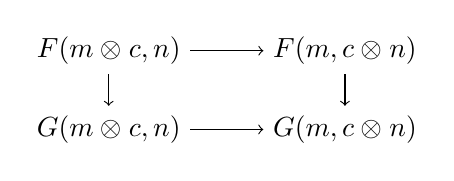
\begin{tikzpicture}
	\node (LT) at (0, 1) {$F(m \otimes^{\cM} c, n)$};
	\node (LB) at (0, 0) {$G(m \otimes^{\cM} c, n)$};
	\node (RT) at (3, 1) {$F(m, c \otimes^{\cN} n)$};
	\node (RB) at (3, 0) {$G(m, c \otimes^{\cN} n)$};
	\draw [->] (LT) -- node [left] {$$} (LB);
	\draw [->] (LT) -- node [above] {$$} (RT);
	\draw [->] (RT) -- node [right] {$$} (RB);
	\draw [->] (LB) -- node [below] {$$} (RB);
	%\node at (0.5, 1) {$\ulcorner$};
	%\node at (1.5, 0.5) {$\lrcorner$};
\end{tikzpicture}.
\end{center}
\end{definition}

\begin{definition}
	Let $\cM$ be a right $\cC$-module category and let $\cN$ be a left $\cC$-module category. The {\em balanced tensor product} is a linear category $\cM \boxtimes_{\cC} \cN$
	 together with a $\cC$-balanced right exact bilinear functor $\boxtimes_{\cC} : \cM \times \cN \to \cM \boxtimes_{\cC} \cN$, such that for all linear categories $\cD$, the functor $\boxtimes_{\cC}$ induces an equivalence between the category of $\cC$-balanced right exact bilinear functors $\cM \times \cN \to \cD$ and the category of right exact linear functors $\cM \boxtimes_{\cC} \cN \to \cD$.
\end{definition}
\nid More succinctly, we might say, the balanced tensor product $\cM \boxtimes_{\cC} \cN$ corepresents $\cC$-balanced right exact bilinear functors out of $\cM \times \cN$.  The balanced tensor product is also known as the ``relative Deligne tensor product", because the (unbalanced) tensor product $\cM \boxtimes \cN$ of linear categories is often called the ``Deligne tensor product".  

If it exists, the balanced tensor product is unique up to equivalence, and this equivalence is in turn unique up to unique natural isomorphism. Said another way, the 2-category of linear categories representing the balanced tensor product is either contractible or empty. 

Etignof--Nikshych--Ostrik \cite{0909.3140} established the existence of the balanced tensor product of semisimple module categories over semisimple tensor categories over a field of characteristic zero.  A construction of the balanced tensor product for finite tensor categories satisfying the additional assumption that $\cM \boxtimes \cN$ is exact as a $\cC$-bimodule category can be extracted from \cite[Thm 3.1]{1102.3411}.  Note that the proof of the existence of the balanced tensor product outlined in \cite{MR3107567} uses the rigidity and finiteness assumptions in essential ways, but (despite \cite[Note 2.7]{MR3107567}) does not use exactness.  

We give an alternative construction of the balanced tensor product for finite tensor categories.

\begin{theorem} \label{thm:DelignePrdtOverATCExists}
	Let $\cC$ be a finite tensor category and let $\cM_{\cC}$ and ${}_{\cC}\cN$ be finite right and left $\cC$-module categories, respectively. Assume that the action of $\cC$ on $\cM$ and the action of $\cC$ on $\cN$ are right exact in the $\cC$-variable.
	\begin{enumerate}
		\item The balanced tensor product $\cM \boxtimes_{\cC} \cN$ exists and is a finite linear category.
		\item If $\cM = \Mod{A}{}(\cC)$ and $\cN = \Mod{}{B}(\cC)$, then $\cM \boxtimes_{\cC} \cN \simeq \Mod{A }{B}(\cC)$, the category of $A$--$B$-bimodule objects in $\cC$.
		\item The functor $\boxtimes_{\cC}: \cM \times \cN \to \cM \boxtimes_{\cC} \cN$ is exact in each variable and satisfies 
		\begin{equation*}
			 \Hom_{\cM \boxtimes_{\cC} \cN} (x \boxtimes_{\cC} y, x' \boxtimes_{\cC} y') \cong \Hom_{\cC}(1, \IHom_{\cM}(x,x') \otimes \IHom_{\cN}(y, y'))
		\end{equation*}
		\item Given exact $\cC$-module functors $F_0: M \to M'$ and $F_1: N \to N'$, the $\cC$-balanced functor $F: M \times N \to M' \times N' \to M' \boxtimes_{\cC} N'$ induces an exact functor $\overline{F}: M \boxtimes_{\cC} N \to M' \boxtimes_{\cC} N'$.
	\end{enumerate} 
\end{theorem}


\begin{proof}  
	 By Theorem \ref{thm:EGNO2.11.6}, there exist algebra objects $A, B \in \cC$ and equivalences $\cM \simeq \Mod{A}{}(\cC)$ and $\cN \simeq \Mod{}{B}(\cC)$. The linear category $\Mod{A }{B}(\cC)$ is finite by Lemma~\ref{lem:recognizefinitecats} (using the free-forgetful adjunction to $\cC$).  Thus (2) implies (1).
	 
	 By Lemma \ref{lma:RigidIsExact}, the tensor product functor
	\begin{equation*}
		\cM \times \cN \simeq \Mod{A}{}(\cC) \times  \Mod{}{B}(\cC) \to \Mod{A}{B}(\cC)
	\end{equation*}
	is exact in each variable separately.  This bilinear functor is also $\cC$-balanced by the associator of $\cC$. Moreover we have
	\begin{align*}
		&\Hom_{\cC}(1, \IHom_{\cM}(x,x') \otimes \IHom_{\cN}(y, y')) \\
		& = \Hom_{\cC}(1, \IHom_{\Mod{A}{}}(x,x') \otimes \IHom_{\cN}(y, y')) \\
		&\cong \Hom_{\cC}(1, \IHom_{\Mod{A}{}}(x,x' \otimes \IHom_{\cN}(y, y')) ) \\
		& \cong \Hom_{\Mod{A}{}}(x, x' \otimes \IHom_{\cN}(y, y') ) \\
		& = \Hom_{\Mod{A}{}}(x, x' \otimes \IHom_{\Mod{}{B}}(y, y') )\\
		& \cong \Hom_{\Mod{A}{}}(x,  \IHom_{\Mod{}{B}}(y, x' \otimes y') )\\
		& \cong \Hom_{\Mod{A}{B}}(x \otimes y, x' \otimes y')
	\end{align*} 
where the second and fifth isomorphisms use the fact that the enriched hom is a $\cC$-module functor (see Lemma~\ref{lma:module-adjoint}). This establishes the formula in (3), and so $(2)$ implies $(3)$.

	We now prove (2), and then later establish (4).  We wish to show that for any linear category $\cD$ the category of right exact functors 
\begin{equation*}
	\overline{F}:\Mod{A}{B}(\cC) \to \cD
\end{equation*}
	is naturally equivalent to the category of $\cC$-balanced functors $F:\cM \times \cN \to \cD$ that are right exact in each variable separately. Every functor of the former type certainly restricts to one of the later type; we must show that a functor of the latter type extends uniquely (up to canonical isomorphism) to one of the former type. 
	
The key observation is that every object of $\Mod{A}{B}(\cC)$ may be functorially written as a coequalizer of objects in the image of $\cM \times \cN$. Specifically, for any $X \in \Mod{A}{B}(\cC)$, we have the coequalizer:
\begin{equation*}
%	{}_A A \otimes A \otimes X_B \rightrightarrows {}_A A \otimes X_B \to {}_A X_B.
	{}_A X \otimes B \otimes B_B \rightrightarrows {}_A X \otimes B_B \to {}_A X_B.
\end{equation*}
Let %$\delta: {}_A A \otimes A \otimes X_B \to {}_A A \otimes X_B$ 
$\delta: {}_A X \otimes B \otimes B_B \to {}_A X\otimes B_B$ 
be the difference of the two maps in the coequalizer. 
For any right exact functor $\overline{F}: \Mod{A}{B}(\cC) \to \cD$, the value $\overline{F}({}_A X_B)$ is canonically determined as a cokernel:
\begin{equation*}
%	\overline{F}({}_A X_B) = \coker \left( \overline{F}(\delta): \overline{F}({}_A A \otimes A \otimes X_B) \to \overline{F}({}_A A \otimes X_B) \right).
	\overline{F}({}_A X_B) = \coker \left( \overline{F}(\delta): \overline{F}( {}_A X \otimes B \otimes B_B) \to \overline{F}({}_A X \otimes B_B) \right).
\end{equation*} 
	
Suppose we are given a $\cC$-balanced functor $F:\cM \times \cN \to \cD$ that is right exact in each variable separately. It is tempting to try to define the extension $\overline{F}: \Mod{A}{B}(\cC) \to \cD$ via a formula of the type:
\begin{equation*}
%	``\overline{F}({}_A X_B) := \coker \left( F(\delta): F({}_A A \otimes A,  X_B) \to {F}({}_A A , X_B) \right)."
	``\overline{F}({}_A X_B) := \coker \left( F(\delta): F( {}_A X, B \otimes B_B) \to F({}_A X, B_B) \right)."
\end{equation*} 
The difficulty is that while the relevant objects are in the image of $\cM \times \cN$, the map $\delta$ is not. 
Yet for each $X \in \Mod{A}{B}(\cC)$ we may define a map $\overline{\delta}_X$ as the difference between the composite of the balancing isomorphism and the action of $B$ on $X$,
\begin{equation*}
F( {}_A X, B \otimes B_B) \cong F({}_A X \otimes B, B_B) \to F({}_A X, B_B),
\end{equation*}
and the action of $B$ on itself,
\begin{equation*}
F( {}_A X, B \otimes B_B) \to F({}_A X, B_B).
\end{equation*}
The desired extension can then be defined as $\overline{F}({}_A X_B) := \coker(\overline{\delta}_X)$.
%%shown in Figure %\ref{fig:RelDelingePdtDiagram}.
%%\begin{figure}[htbp]
%	\begin{center}
%		\begin{tikzpicture} \matrix (m) [matrix of math nodes, row sep={1.5cm,between origins}] {
%		 F({}_AA \otimes A \otimes X, B \otimes B_B) &[1cm] F({}_AA \otimes X, B \otimes B_B) &[1cm] F({}_A X, B \otimes B_B) &[0.5cm] 0 \\
%		F({}_AA \otimes A, X \otimes B \otimes B_B) & F({}_AA, X \otimes B \otimes B_B) & & \\
%		F({}_AA \otimes A, X \otimes B_B) & F({}_AA , X \otimes B_B) & & \\
%		 F({}_AA \otimes A \otimes X, B_B) & F({}_AA \otimes X, B_B) & F({}_AX,B_B)  & 0 \\
%		& &\coker(\overline{\delta}_X)  & \\
%			};
%			\draw [->] (m-1-1) -- node [above] {$\delta_1$} (m-1-2);
%			\draw [->] (m-1-2) -- node [above] {$$} (m-1-3);
%			\draw [->] (m-1-3) -- node [above] {$$} (m-1-4);
%			\draw [->] (m-4-1) -- node [above] {$\delta_1$} (m-4-2);
%			\draw [->] (m-4-2) -- node [above] {$$} (m-4-3);
%			\draw [->] (m-4-3) -- node [above] {$$} (m-4-4);
%			\draw [->] (m-1-1) -- node [left] {$\cong$} (m-2-1);
%			\draw [->] (m-1-2) -- node [left] {$\cong$} (m-2-2);
%			\draw [->] (m-3-1) -- node [left] {$\cong$} (m-4-1);
%			\draw [->] (m-3-2) -- node [left] {$\cong$} (m-4-2);
%			\draw [->] (m-2-1) -- node [left] {$\delta_2$} (m-3-1);
%			\draw [->] (m-2-2) -- node [left] {$\delta_2$} (m-3-2);
%			\draw [->,dashed] (m-1-3) -- node [left] {$\overline{\delta}_X$} (m-4-3);
%			\draw [->,dashed] (m-4-3) -- node [left] {$$} (m-5-3);
%			\node [node distance = 1.75cm, right of= m-5-3] {$=:\overline{F}({}_AX_B)$};
%		\end{tikzpicture}
%	\end{center}
%%	\caption{A digram useful for demonstrating the existence of the balanced tensor product.}
%%	\label{fig:RelDelingePdtDiagram}
%%\end{figure}
%Here the arrows labeled with isomorphisms come from the $\cC$-balanced structure of the functor $F$, while the remaining solid arrows are maps in the image of $\cM \times \cN$. The maps labeled with either $\delta_1$ or $\delta_2$ represent difference maps of maps in $\cM$ or $\cN$, as above.  (The fact that this diagram commutes uses the coherence and naturality of the $\cC$-balanced structure. To verify the commutativity it is easiest to break each difference map into its constituent piece (one from the multiplication in either $A$ or $B$, and one from the action on $X$) and to show commutativity with respect to these maps.)
%The rows of this diagram are exact (since $F$ was assumed to be right exact in each variable) and hence this diagram defines a unique map $\overline{\delta}_X$, shown as the long dashed arrow. We may define the value of the extension $\overline{F}$ on the object ${}_AX_B$ as the cokernel of $\overline{\delta}_X$. 
We leave it to the reader to verify that this extension gives a well-defined right exact functor 
\begin{equation*}
	\overline{F}: \Mod{A}{B}(\cC) \to \cD,
\end{equation*} 
and implements the desired equivalence between such right exact functors and $\cC$-balanced exact-in-each-variable functors. Verifying that this construction is well defined makes use of the pentagon identity satisfied by $\cC$-balanced functors. This establishes (1), (2), and (3). 

We now prove the final property (4). By Theorem \ref{thm:EGNO2.11.6}, there exist algebra objects $A, B, A'$, and $B' \in \cC$ and equivalences $\cM \simeq \Mod{A}{}(\cC)$, $\cN \simeq \Mod{}{B}(\cC)$, $\cM' \simeq \Mod{A'}{}(\cC)$, and $\cN \simeq \Mod{}{B'}(\cC)$. Since $F_0$ and $F_1$ are right exact, they are equivalent to tensoring with bimodules:
\begin{align*}
	F_0(-) &\cong {}_{A'}x \otimes_A (-); \\
	F_1(-) & \cong (-) \otimes_B y_{B'}.
\end{align*}
Since $F_0$ and $F_1$ are exact, we may call these modules {\em flat} over $A$ or $B$, respectively. We wish to show that the induced functor:
\begin{equation*}
	\overline{F}(-) = {}_{A'}x \otimes_A (-) \otimes_B y_{B'}: \Mod{A}{B}(\cC) \to \Mod{A'}{B'}(\cC)
\end{equation*}
is exact. Since the forgetful functor $U: \Mod{A'}{B'}(\cC) \to \cC$ is exact and reflects short exact sequences, it is enough to show that 
\begin{equation*}
	x \otimes_A (-) \otimes_B y: \Mod{A}{B}(\cC) \to \cC
\end{equation*}
is exact. Let $0 \to m \to m' \to m'' \to 0$ be a short exact sequence of $A$--$B$-bimodules. After tensoring with $x$ on the left we obtain a sequence of right $B$-modules:
\begin{equation*}
	0 \to x \otimes_A m \to x \otimes_A m' \to x \otimes_A {m''} \to 0
\end{equation*}
Since $x$ is flat, this sequence is exact after forgetting the $B$-module structure. Hence it is also an exact sequence of $B$-modules. Thus, since $y$ is flat, we obtain an exact sequence
\begin{equation*}
		0 \to x \otimes_A m \otimes_B y \to x \otimes_A m'\otimes_B y \to x \otimes_A {m''}  \otimes_B y \to 0
\end{equation*}
	as desired. 
%The final property, part (4), now follows from a routine diagram chase, which we also leave to the reader. 
\end{proof}

\begin{remark}
The balanced (Deligne) tensor product, constructed above for finite module categories over a finite tensor category, may fail to exist without the finiteness assumptions---see Lopez Franco \cite{1212.1545} for a counterexample, even in the unbalanced case.  A balanced tensor product does exist a bit more generally, though.  Recall that a finitely cocomplete $k$-additive category is a category that is $\overline{\Vect}_k$-enriched and that admits all finite colimits.  Right exact functors between such categories are, by definition, those that preserve finite colimits.  The balanced ``Kelly" tensor product of finitely cocomplete $k$-additive module categories (over a rigid finitely cocomplete $k$-additive tensor category) corepresents balanced right exact bilinear functors into finitely cocomplete $k$-additive categories.  Unlike the Deligne tensor product, the Kelly tensor product always exists---see \cite{MR651714, MR648793} for the unbalanced case and \cite[Rmk~3.21]{1501.04652} for the balanced case.  Lopez Franco \cite{1212.1545} shows that when the unbalanced Deligne tensor product exist, it is equivalent to the Kelly tensor product.

The proof of the preceding theorem shows that when $\cC$ is a finite tensor category, and $\cM_{\cC}$ and ${}_{\cC}\cN$ are finite right and left $\cC$-module categories, the balanced Deligne tensor product is equivalent to the balanced Kelly tensor product.  This equivalence follows because the proof that $\Mod{A}{B}(\cC)$ corepresents $\cC$-balanced functors into linear categories just as well shows that $\Mod{A}{B}(\cC)$ corepresents $\cC$-balanced functors into finitely cocomplete $k$-additive categories.  (In the displayed commutative diagram, when the target category $\cD$ is not abelian but merely additive, the rows are `exact' in the sense that they are cokernel sequences.)
\end{remark}

\begin{remark}
The construction of the balanced tensor product outlined in~\cite{MR3107567} expresses the tensor $\cM \boxtimes_{\cC} \cN$ as a category of right exact $\cC$-module functors.  The expression~\cite[Eq~13]{MR3107567} for this functor category is cited from~\cite{0909.3140}, and in both places is appropriate for the balanced tensor of module categories but is not quite correct for the balanced tensor of bimodule categories (being off by a twist by a double dual functor).  The functor category that is a balanced tensor product for bimodule categories is $\mathrm{Fun}_{\cC\textrm{-}\mathrm{mod}}^{\mathrm{r.e.}}(\cM^{\ast},\cN)$, where the $\cC$--$\cD$-bimodule category $\cM^{\ast}$ has underlying linear category $\cM^{\mathrm{op}}$, with the left action by an object $c \in \cC$ given by acting on the right by the \emph{left} dual object ${}^{\ast} c \in \cC$ and the right action by an object $d \in \cD$ given by acting on the left by the \emph{left} dual object ${}^{\ast} d \in \cD$.  This functor-category description of the balanced tensor is related to our bimodule description as follows: when $\cM = \Mod{A}{}(\cC)$ and $\cN = \Mod{}{B}(\cC)$, there is a functor equivalence $\Mod{A}{B}(\cC) \ra \mathrm{Fun}_{\cC\textrm{-}\mathrm{mod}}^{\mathrm{r.e.}}(\cM^{\ast},\cN)$ taking a bimodule object ${}_A X_B$ to the functor that takes the object $m \in \cM = \Mod{A}{}(\cC)$ viewed as an object of $\cM^{\ast}$ to the object $m^\ast \otimes_A X \in \Mod{}{B}(\cC) = \cN$, where $m^\ast$ is the right dual of $m$ viewed as an object of $\cC$.
\end{remark}

\begin{example}
Let $\Vect[K]$ denote the category of $K$-graded vector spaces for a finite group $K$.  The balanced product $\Vect \boxtimes_{\Vect[K]} \Vect$ is the category of $k[K]$-bimodules in $\Vect[K]$. The category of $k[K]$-modules in $\Vect[K]$ is equivalent to $\Vect$, so the $k[K]$-bimodules in $\Vect[K]$ can be identified with $\text{mod-}(k[K]) \cong \Rep(K)$.
\end{example}

\begin{remark}
	If ${}_{\cD}\cM_{\cC}$ and ${}_{\cC}\cN_{\cE}$ are bimodule categories, then the actions of $\cD$ and $\cE$ induce a $\cD$--$\cE$-bimodule category structure on $\cM \boxtimes_{\cC} \cN$. This bimodule category satisfies the analogous universal property for $\cC$-balanced bilinear bimodule functors.
\end{remark}

\begin{remark}
The above theorem assumes that $\cC$ is a finite tensor category, that is a finite rigid linear monoidal category.  The non-balanced tensor product can be defined substantially more generally \cite{1212.1545}, and we hope that the balanced tensor product can also be defined more generally.
\end{remark}

Part (2) of the above theorem expresses the balanced tensor product of two module categories $\cM = \Mod{A}{}(\cC)$ and $\cN = \Mod{}{B}(\cC)$ as a category of bimodules $\cM \boxtimes_\cC \cN \simeq \Mod{A}{B}(\cC)$.  When the tensor category $\cC$ is merely $\Vect$, this expresses the ordinary tensor product $\Mod{}{A}(\Vect) \boxtimes \Mod{}{B}(\Vect)$ of two categories of modules again as a category of modules, $\Mod{}{(A \otimes B)}(\Vect)$.  More generally, the ordinary tensor product of two categories of modules in any tensor categories is again a category of modules, as follows.

\begin{proposition}
	%\label{lem:}
	If $\cN = \Mod{}{B}(\cC)$ and $\cP = \Mod{}{C}(\cD)$, for algebra objects $B \in \cC$ and $C \in \cD$, then $$\cN \boxtimes \cP \simeq \Mod{}{(B \boxtimes C)}(\cC \boxtimes \cD)$$ as a left $\cC \boxtimes \cD$-module category.
\end{proposition}

\begin{proof}
	The forgetful functors from $\cN$ to $\cC$ and $\cP$ to $\cD$ are part of monadic adjunctions:
	\begin{align*}
		(-) \otimes B_{B}:\cC \rightleftarrows \cN = \Mod{}{B}(\cC): U \\
		(-) \otimes C_{C}:\cD \rightleftarrows \cP = \Mod{}{C}(\cD): U
	\end{align*}
	Since both functors in the adjunction are right exact (the forgetful functor is exact, not just left exact) these adjunctions descend to an adunction between the tensor products. 
	\begin{equation*}
		(-) \otimes (B \boxtimes C)_{B \boxtimes C}: \cC \boxtimes \cD \rightleftarrows \cN \boxtimes \cP: \overline{U}.
	\end{equation*}
	Any $\cC \boxtimes \cD$-module functor from $\cC \boxtimes \cD$ to itself is given by tensoring by an object in $\cC \boxtimes \cD$, hence any monad on $\cC \boxtimes \cD$ that is compatible with the module actions comes from an algebra in $\cC \boxtimes \cD$.  Hence we need only show that this adjunction is monadic.  
		
	By the the crude monadicity theorem \cite[\S~3.5]{MR771116} we only need to show that $\overline{U}$ reflects isomorphisms and $\overline{U}$ preserves coequalizers of reflexive pairs.  Observe that the individual functors (both called $U$) have these properties. Moreover everything in $\cN$ is a coequalizer of objects in the image of $\cC$, everything in $\cP$ is a coequalizer of objects in the image of $\cD$, and everything in $\cN \boxtimes \cP$ is a coequalizer of objects in the image of $\cN \times \cP$. Thus it follows that every object in $\cN \boxtimes \cP$ is a coequalizer of objects in the image of $\cC \times \cD$. For such objects $\overline{U}$ reflects isomorphisms, since the original $U$ do so. Hence, by the five lemma, it follows that $\overline{U}$ reflects isomorphisms. 

For the latter property we will in fact show that $\overline{U}$ preserves all coequalizers. Since our categories are additive the coequalizer of $f$ and $g$ is the cokernel of $(f-g)$.  Thus it is sufficient to show that $\overline{U}$ is exact and hence that $\overline{U}$ preserves cokernels.  The exactness of $\overline{U}$ follows from Part (4) of Theorem~\ref{thm:DelignePrdtOverATCExists} and exactness of the original forgetful functors $U$.  
\end{proof}


\bibliographystyle{alpha}
\bibliography{dtcbib}
\end{document}




